\section{Diskussion}
\label{sec:Diskussion}
Der Literaturwert vom Brechungsindex von Silizium liegt bei 
\begin{equation*}
  n=3.35
\end{equation*}
für eine Wellenlänge von $\lambda=633\ \textrm{nm}$. Wird dieser Wert mit den experimentellen Werten aus \autoref{sec:Auswertung} verglichen, ergben sich die Abweichungen
\begin{align*}
  n_{\bot_\%}&=32.4\ \%\\
  n_{\|_\%}&=22.1\ \%\\
  n_{\alpha_{p_\%}}&=2.4\ \%
\end{align*}
für die Brechungsindizes. Die Abweichung durch den Brewster-Winkel ist gering und noch im Rahmen. Die Abweichungen des Brechungsindex bei dessen Berechnung mit der paralleln und senkrechten Polarisation ist viel zu hoch. Diese Abweichung kann durch das einfallende Licht von außen, das ungenaue justieren des Goniometers, den falschen gemessene Bruchteil des Lasers im Detektor, einen fehlerhaften Spiegel, den falschen oder ungenau ausgewählten Winkel im Polarisator, einer lockeren Stellschraube oder Klemmschraube und dem falschen Ablesen von Messwerten auf dem Amperemeter entstehen, wobei hier das Zweit- und Letztgenannte wahrscheinlich ein Grund für die Abweichung sein kann. Allerdings war die Abweichung beim Brewster-Winkel so gering, das anzunehmen ist, dass eventuell das Amperemeter nicht mehr richtig funktioniert. 

\section{Literaturverzeichnis} 
[1] Technische Universität Dortmund, \textit{V407: Fresnel Formeln}\\

[2] Literaturwert für den Brechungsindex von Silizium. 2022.\\ 
URL: https://www.korth.de/material/detail/Silizium (besucht am 15.05.2022).


\section{Anhang}
\label{sec:a}
\begin{figure}[H]
  \centering
  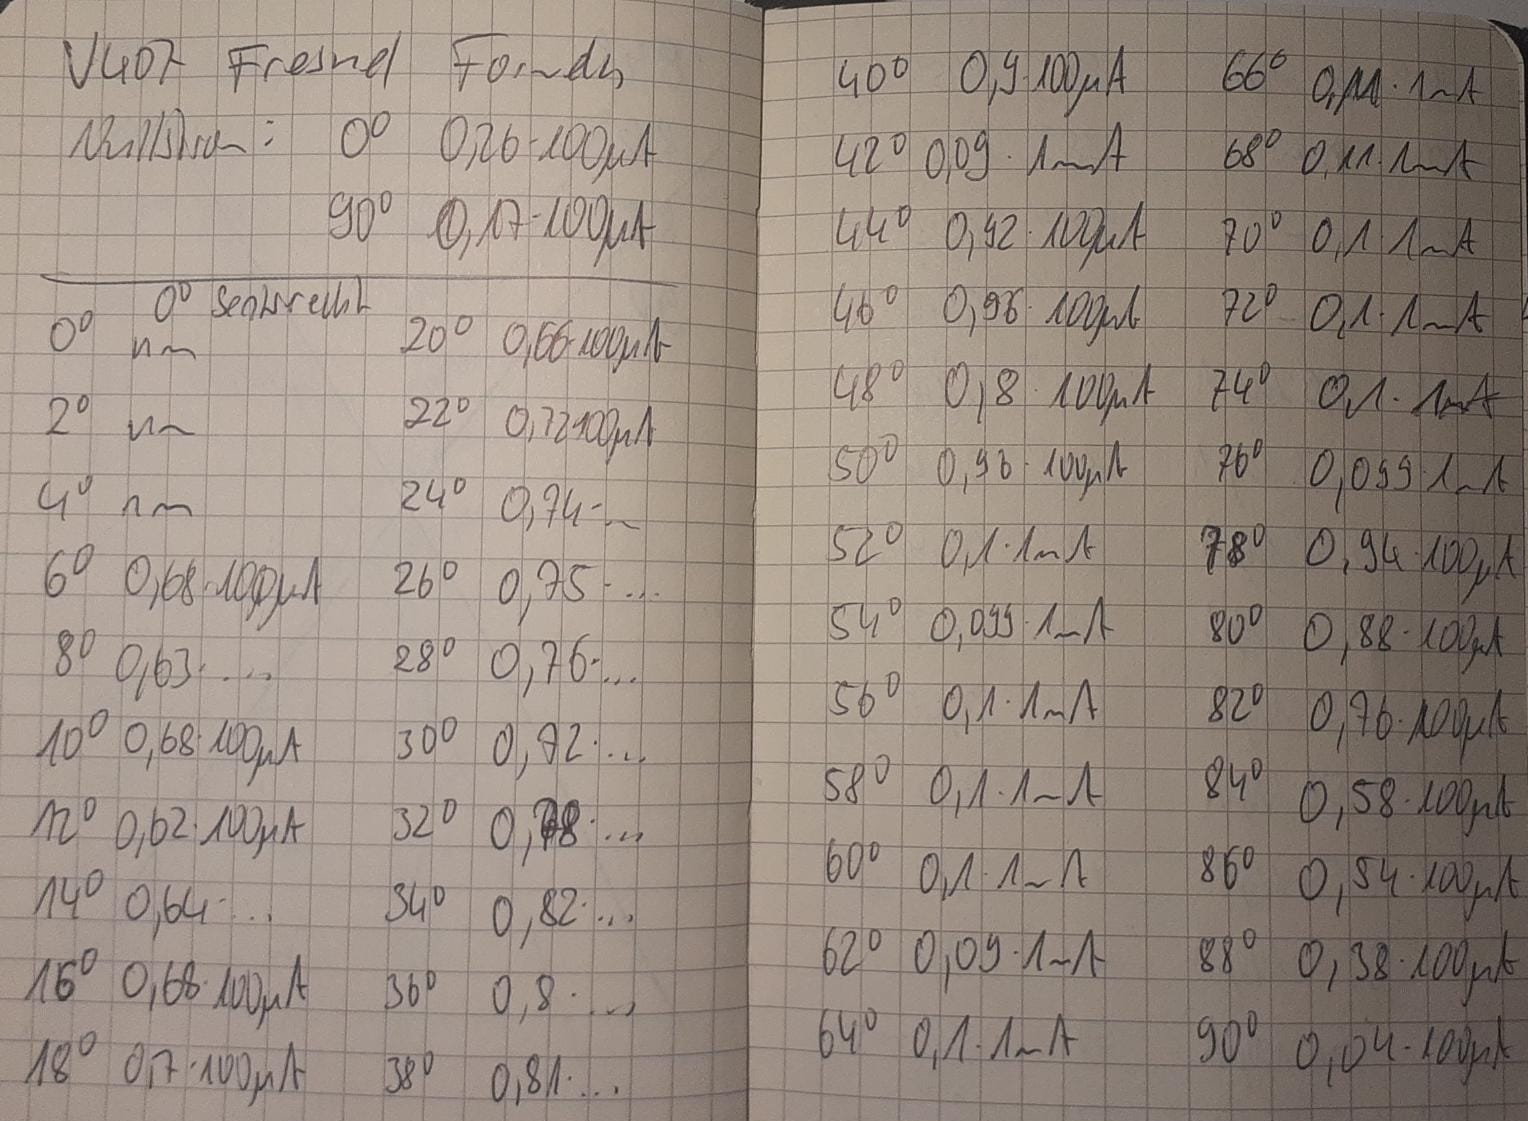
\includegraphics[width=9cm]{a1.png}
  \caption{Originale Messdaten.}
\end{figure}
\begin{figure}[H]
  \centering
  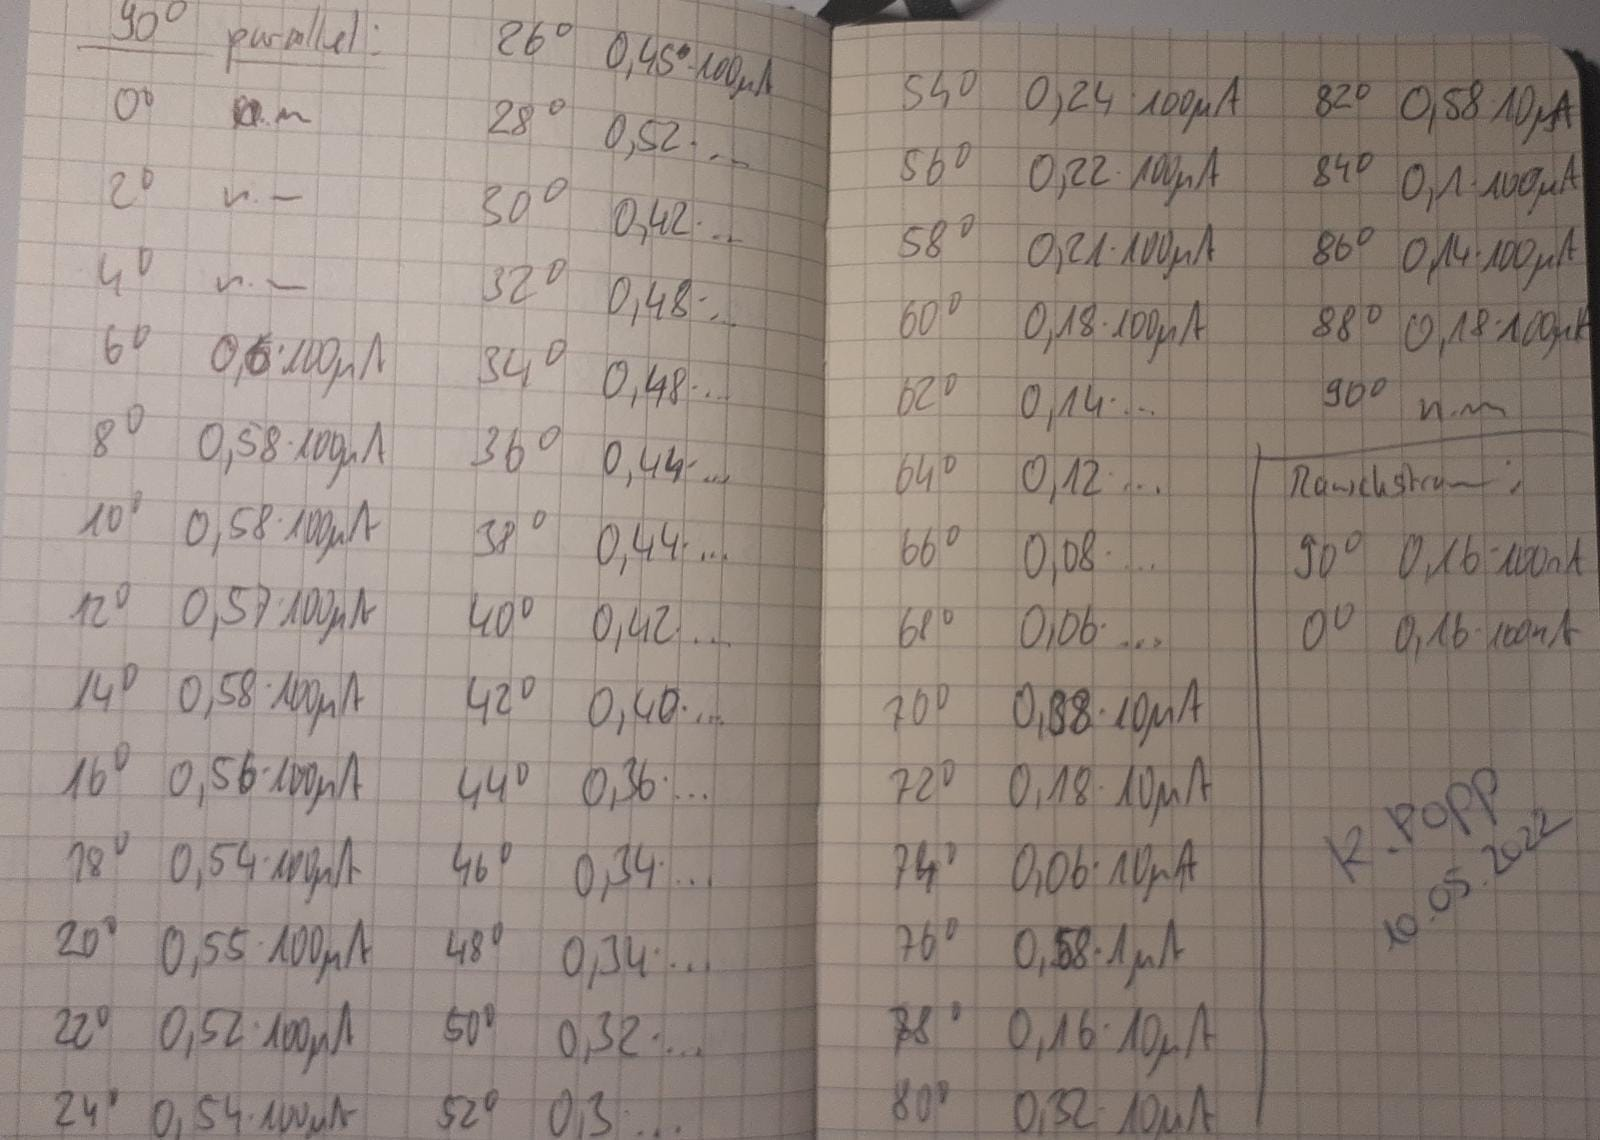
\includegraphics[width=9cm]{a2.png}
  \caption{Originale Messdaten.}
\end{figure}
\end{document}
